\documentclass[11pt]{exam}

%%%%%%%%%%%%%%%%%%%%%%%%%% Preamble %%%%%%%%%%%%%%%%%%%%%%%%%% 
\input{Admin/1. Packages}
\input{Admin/2. WEB Course Info}
\input{Admin/3. WEB Outcomes}
\input{Admin/4. Commands}
\input{Admin/8. Fonts}

%%%%%%%%%%%%% Exam Information  %%%%%%%%%%%%%%%%%%%%%%%%%% 

\newcommand{\exam}{Midterm Exam}
\newcommand{\TimeLimit}{2 hours}

\begin{document}

%%%% Show/Don't Show Points %%%% 
\addpoints
% \pointformat{}
% \nopointsmargin

%%%% Show/Don't Show Solutions %%%% 
%\printanswers
\noprintanswers

%%%%%%%%%%%%%%%%%%%%%%%%%% Scratch Paper %%%%%%%%%%%%%%%%%%%%%%%%%%
\blankpage

%%%%%%%%%%%%%%%% Cover Page %%%%%%%%%%%%%%%% 
\input{Admin/6. CoverPage}

\newpage

%%%% Questions %%%%
\begin{questions}
\headerbox{\occ}
\question[10] \textbf{\textit{Without solving}}, use the discriminant to determine the number and the type of the solutions.
Determine the number and type of solutions for the following equation: 

 \(-4 \, x^{2} - 9 = x\) 

\begin{solution}
\(-4x^2 + (-1)x + -9 = 0\) 

 \(\Delta = (-1)^2 - 4(-4)(-9)\) 

 \(\Delta = -143\) 

 \(\boxed{\text{ two solutions, complex conjugate roots }}\)
\end{solution} \vspace{\stretch{3}}\\
number of solutions: \fillin[][.75in] \hspace{.25in} type of solutions: \fillin[][2.5in]

\question[5] A quadratic function has the characteristics given below. Use the axis of symmetry to generate two additional points, then use all five points to graph the function.
\vspace{.25in}

\begin{multicols}{2}
\begin{itemize}
\item
\(\text{Vertex: } (-2, -9)\)

\item
\(x\text{-intercept: } -5\)

\item
\(y\text{-intercept: } -5\)

\end{itemize}
\columnbreak
\centering
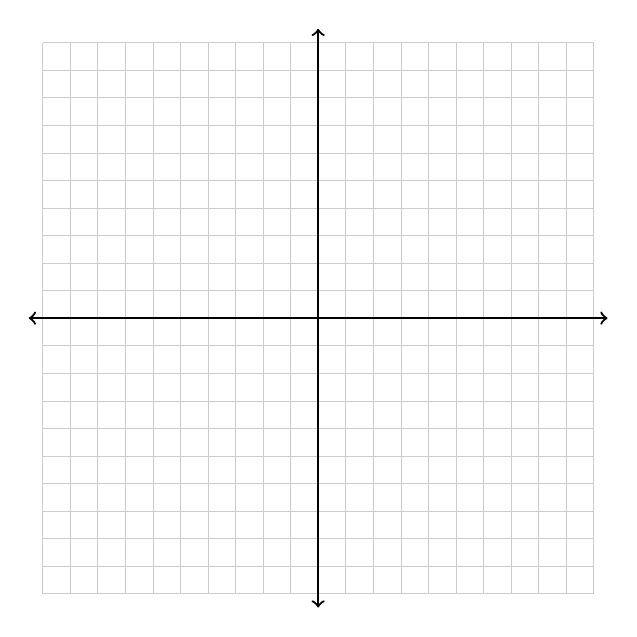
\begin{tikzpicture}[scale=0.35] \draw[step=1cm, gray!40, very thin] (-10,-10) grid (10,10); \draw[thick, <->] (-10.5,0) -- (10.5,0); \draw[thick, <->] (0,-10.5) -- (0,10.5); \end{tikzpicture}
\end{multicols}

\begin{solution}
\begin{multicols}{2}  

\begin{itemize}
\item
\(\text{Vertex: } (-2, -9)\)

\item
\(y\text{-intercept: } (0, -5)\)

\item
\(\text{Reflected } y\text{-int: } (-4, -5)\)

\item
\(\text{Given Root: } (-5, 0)\)

\item
\(\text{Reflected Root: } (1, 0)\)

\end{itemize}
 \columnbreak  

 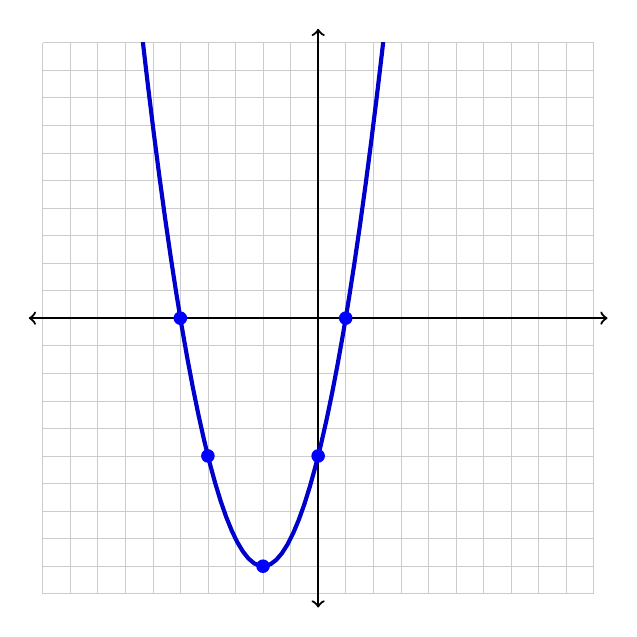
\begin{tikzpicture}[scale=0.35] \draw[step=1cm, gray!40, very thin] (-10,-10) grid (10,10); \draw[thick, <->] (-10.5,0) -- (10.5,0); \draw[thick, <->] (0,-10.5) -- (0,10.5); \clip (-10,-10) rectangle (10,10); \draw[line width=1.5pt, blue!80!black, samples=100, domain=-10:10, <->] plot (\x, {1.0*(\x - -2)^2 + -9}); \fill[blue] (-2,-9) circle (7pt); \fill[blue] (-5,0) circle (7pt); \fill[blue] (1,0) circle (7pt); \fill[blue] (0,-5) circle (7pt); \fill[blue] (-4,-5) circle (7pt); \end{tikzpicture} 

 \end{multicols}
\end{solution}
 \vspace{\stretch{1}}

\newpage
\question[5] Find the vertex, axis of symmetry, $x$- and $y$- intercepts, domain, and range for the function 

 \(f(x) = \frac{1}{2}(x - 6) 

 
\renewcommand{\arraystretch}{3}
\begin{center}
\begin{tabular}{|l|l|}
\hline
vertex & \hspace{175px} \\ \hline
axis of symmetry & \\ \hline
$x$-intercepts(s) & \\ \hline
$y$-intercept & \\ \hline
domain & \\ \hline
range & \\ \hline
\end{tabular}
\end{center}
 

 \begin{solution}
\(\textbf{Direction: } \text{Opens Up}\) 

 \(\textbf{Vertex: } (6, -18)\) 

 \(\textbf{Axis of Symmetry: } x = 6\) 

 \(\textbf{x-intercepts:}\) 

 \(\frac{1}{2}(x - 6)^2 -18 = 0\) 

 \((x - 6)^2 = 36\) 

 \(x = 6 \pm 6\) 

 \(\boxed{ 0, 12 }\) 

 \(\textbf{y-intercept:}\) 

 \(= \frac{1}{2}(0 - 6)^2 -18\) 

 \(= \frac{1}{2}(36) -18\) 

 \(= 18 -18\) 

 \(\boxed{ 0 }\) 

 \(\textbf{Domain: } (-\infty, \infty)\) 

 \(\textbf{Range: } [-18, \infty)\)
\end{solution}

\newpage
\question Suppose a rocket carrying fireworks is launched from a hill 59 feet above a lake. The rocket's height \(h\) (in feet) above the lake at time \(t\) (in seconds) is given by

 \(h(t) = -16t^2 + 128t + 59\)
\begin{parts}
  \part[2] When will the rocket reach its maximum height?

\begin{solution}
\(t = \frac{-128}{2(-16)} = \frac{-128}{-32}\) 

 \(\boxed{t = 4 \text{ sec}}\)
\end{solution}  \vspace{\stretch{1}} \\ \answerline
  \part[2] What is the maximum height the rocket will reach?

\begin{solution}
\(h(4) = -16(4)^2 + 128(4) + 59\) 

 \(= -256 + 512 + 59\) 

 \(\boxed{h = 315 \text{ ft}}\)
\end{solution}  \vspace{\stretch{1}} \\ \answerline
  \part[1] Interpret your results for the previous two questions in one or more complete sentences, including appropriate units.

\begin{solution}
The rocket will reach a maximum height of 315 ft 4 seconds after launch.
\end{solution}  \fillwithlines{1in}
\end{parts} \newpage

\headerbox{\ocg}
\uplevel{In problems \ref{eq_start} through \ref{eq_end}, solve for \textbf{all} solutions. Identify any extraneous solutions.}
\question[10] \label{eq_start} \(x^{2} + 6 \, x + 12 = 0\) 

\begin{solution}
\(x = \frac{-(6) \pm \sqrt{(6)^2 - 4(1)(12)}}{2(1)}\) 

 \(= \frac{-6 \pm \sqrt{36 - 48}}{2}\) 

 \(= \frac{-6 \pm \sqrt{-12}}{2}\) 

 \(= \frac{-6 \pm 2i\sqrt{3}}{2}\) 

 \(= \frac{2(-3 \pm i\sqrt{3})}{2}\) 

 \(\boxed{x = -3 \pm i\sqrt{3}}\) 

 (No extraneous solutions)
\end{solution} \vspace{\stretch{1}}\\\answerline

\newpage
\uplevel{In problems \ref{eq_start} through \ref{eq_end}, solve for \textbf{all} solutions. Identify any extraneous solutions.}
\question[10] \(\sqrt{x + 16} + 3 = 6\) 

\begin{solution}
\(\sqrt{x + 16} = 3\) 

 \(x + 16 = 9\) 

 \(x = 9 - 16\) 

 \(\boxed{x = -7}\) 

 (No extraneous solutions)
\end{solution} \vspace{\stretch{1}}\\\answerline

\newpage
\uplevel{In problems \ref{eq_start} through \ref{eq_end}, solve for \textbf{all} solutions. Identify any extraneous solutions.}
\question[10] \label{eq_end} \(\displaystyle \frac{x}{x + 2} - \frac{2}{(x + 2)(x + 1)} = \frac{6}{x + 1}\) 

\begin{solution}
\(x(x + 1) - 2 = 6(x + 2)\) 

 \(x^{2} - 5 \, x - 14 = 0\) 

 \((x + 2)(x - 7) = 0\) 

 \(x = 7, \quad x = -2\) 

 \(x = -2 \implies \text{Extraneous}\) 

 \(\boxed{x = 7}\)
\end{solution} \vspace{\stretch{1}}\\\answerline \newpage

\headerbox{\ocb}
\question[5] Evaluate the difference quotient, \(\displaystyle{ \frac{f(x+h)-f(x)}{h}}\) , for \(f(x) = 6 \, x^{2} - 1\). 

\begin{solution}
\(f(x+h) = 6(x+h)^2 - 1\) 

 \(= 6(x^2 + 2xh + h^2) - 1\) 

 \(= 6 \, h^{2} + 12 \, h x + 6 \, x^{2} - 1\) 

 \(\displaystyle{\frac{f(x+h)-f(x)}{h} = \frac{ (6 \, h^{2} + 12 \, h x + 6 \, x^{2} - 1) - (6 \, x^{2} - 1) }{h}}\) 

 \(=\displaystyle{ \frac{ 6 \, h^{2} + 12 \, h x }{h}}\) 

 \(= \displaystyle{ \frac{ h(6 \, h + 12 \, x) }{h}}\) 

 \(\boxed{ 6 \, h + 12 \, x }\)
\end{solution} \vspace{\stretch{1}} \\ \answerline \newpage

\question Given \(f(x) = -2 \, x\) and \(g(x) = -3 \, x^{2} - 2\), find the following:
\begin{parts}
  \part[6] \((f \circ g)(x)\)

\begin{solution}
\(f(g(x)) = -2(-3 \, x^{2} - 2)\) 

 \(\boxed{ 6 \, x^{2} + 4 }\) 

ERROR 1: \(g(f(x))\)

 \(= -3(-2 \, x)^2 - 2\) 

 \(= -3(4 \, x^{2}) - 2\) 

 \(\boxed{ -12 \, x^{2} - 2 }\) 

ERROR 2: \(f(x) \cdot g(x)\)

 \(= (-2 \, x)(-3 \, x^{2} - 2)\) 

 \(\boxed{ 6 \, x^{3} + 4 \, x }\)
\end{solution}  \vspace{\stretch{1}} \\ \answerline
  \part[4] \((f \circ f)(x)\)

\begin{solution}
\(f(f(x)) = -2(-2 \, x)\) 

 \(\boxed{ 4 \, x }\)
\end{solution}  \vspace{\stretch{1}} \\ \answerline
\end{parts} \newpage

\question[10] Given that the function is one-to-one, find the inverse function \(f^{-1}(x)\). 

 \(f(x) = \sqrt[3]{x} + 3\) 

\begin{solution}
\(y = f(x) = \sqrt[3]{x} + 3\) 

 \(x = \sqrt[3]{y} + 3\) 

 \(x - 3 = \sqrt[3]{y}\) 

 \((x - 3)^3 = y\) 

 \(y = (x - 3)^3\) 

 \(\boxed{ f^{-1}(x) = (x - 3)^3 }\) 

  

 \(= (x - 3)(x^2 - 6x + 9)\) 

 \(\boxed{ f^{-1}(x) = x^{3} - 9 \, x^{2} + 27 \, x - 27 }\)
\end{solution} \vspace{\stretch{2}}\\\answerline \newpage

\headerbox{\oci}
\question[10] Use the table to identify the transformations described by \(g(x) = f(x + 1) + 2\). Circle the option that applies and fill in the blanks as appropriate to describe the transformations of the given function. If one does not apply, you may leave it blank. Then apply these transformations to the graph of the function shown below. 

 \(\renewcommand{\arraystretch}{3} \begin{array}{|l|l|} \hline \textbf{Horizontal Transformations} & \textbf{Vertical Transformations} \\ \hline \text{Reflection: YES or NO} & \text{Reflection: YES or NO} \\ \hline \text{Dilation: \underline{\hspace{2cm}} times as wide} & \text{Dilation: \underline{\hspace{2cm}} times as tall} \\ \hline \text{Translation: \underline{\hspace{2cm}} units LEFT or RIGHT} & \text{Translation: \underline{\hspace{2cm}} units UP or DOWN} \\ \hline \end{array}\) 

 \noindent\makebox[\textwidth][c]{ \begin{minipage}{0.48\textwidth} \centering 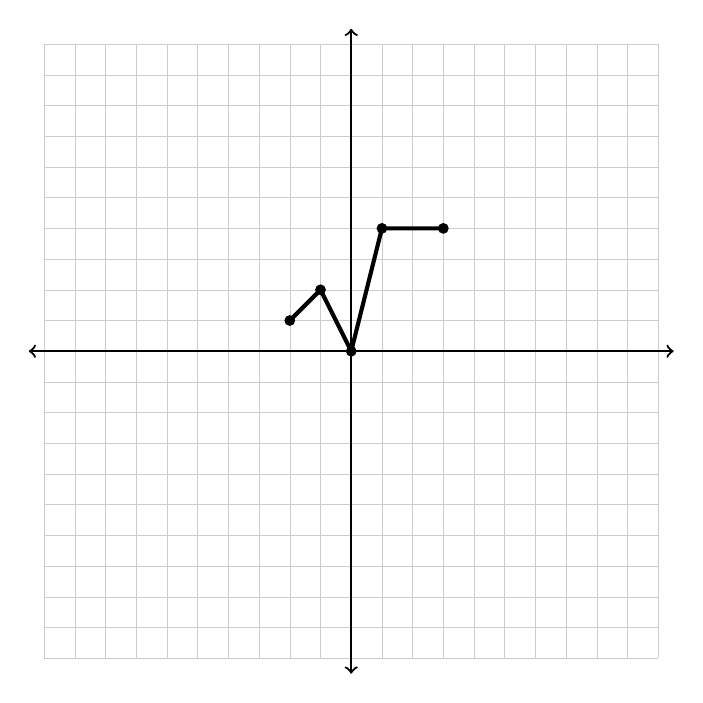
\begin{tikzpicture}[scale=0.39] \draw[step=1cm, gray!40, very thin] (-10,-10) grid (10,10); \draw[thick, <->] (-10.5,0) -- (10.5,0); \draw[thick, <->] (0,-10.5) -- (0,10.5); \draw[line width=1.5pt, black] (-2,1) -- (-1,2) -- (0,0) -- (1,4) -- (3,4);\fill[black] (-2,1) circle (5pt); \fill[black] (-1,2) circle (5pt); \fill[black] (0,0) circle (5pt); \fill[black] (1,4) circle (5pt); \fill[black] (3,4) circle (5pt); \end{tikzpicture} \end{minipage} \hfill \begin{minipage}{0.48\textwidth} \centering 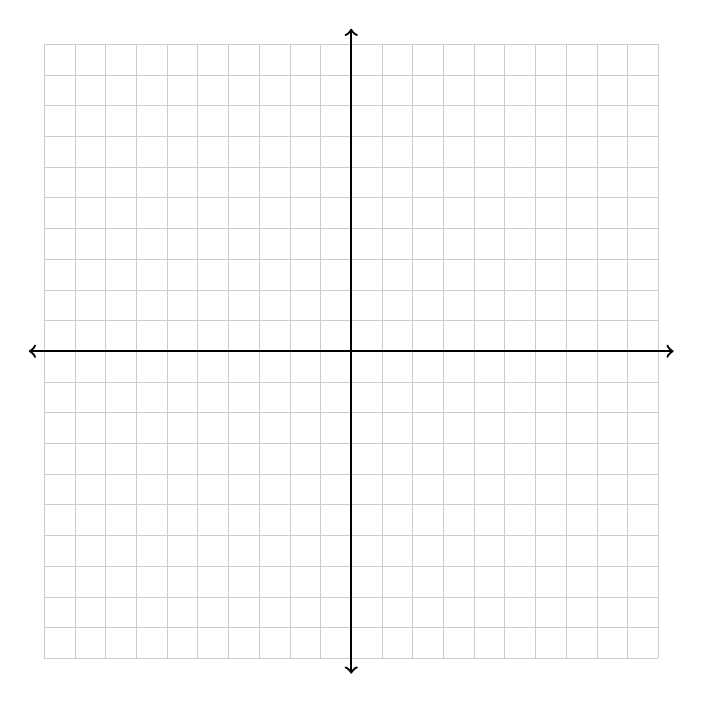
\begin{tikzpicture}[scale=0.39] \draw[step=1cm, gray!40, very thin] (-10,-10) grid (10,10); \draw[thick, <->] (-10.5,0) -- (10.5,0); \draw[thick, <->] (0,-10.5) -- (0,10.5); \end{tikzpicture} \end{minipage} } 

\begin{solution}
\begin{itemize}
\item
 \(\textbf{Horizontal: } \text{Reflection: NO, Dilation: 1, Shift: 1 units LEFT.}\) 

\item
 \(\textbf{Vertical: } \text{Reflection: NO, Dilation: 1, Shift: 2 units UP.}\) 

\end{itemize}


 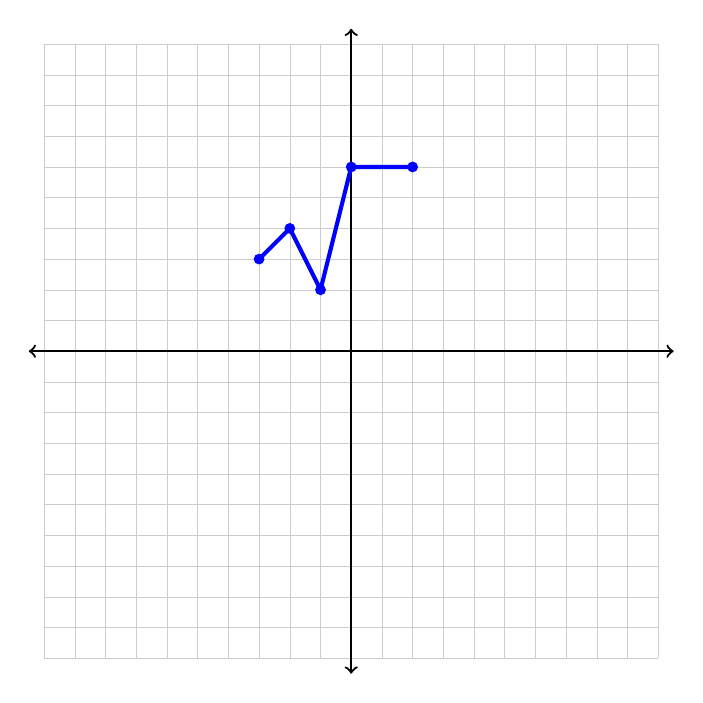
\begin{tikzpicture}[scale=0.39] \draw[step=1cm, gray!40, very thin] (-10,-10) grid (10,10); \draw[thick, <->] (-10.5,0) -- (10.5,0); \draw[thick, <->] (0,-10.5) -- (0,10.5); \draw[line width=1.5pt, blue] (-3,3) -- (-2,4) -- (-1,2) -- (0,6) -- (2,6);\fill[blue] (-3,3) circle (5pt); \fill[blue] (-2,4) circle (5pt); \fill[blue] (-1,2) circle (5pt); \fill[blue] (0,6) circle (5pt); \fill[blue] (2,6) circle (5pt); \end{tikzpicture}
\end{solution} \newpage

\headerbox{\oca}
\question Evaluate the function \(f(x) = 5 \, x^{2} - 8 \, x - 3\).
\begin{parts}
  \part[3] Find \(f(-9)\).

\begin{solution}
\(5(-9)^2 + -8(-9) + -3\)

\(\boxed{f(-9) = 474}\)
\end{solution}  \vspace{\stretch{1}} \\ \answerline
  \part[3] Find \(f(-x)\).

\begin{solution}
\(5(-x)^2 + -8(-x) + -3\)

\(\boxed{f(-x) = 5 \, x^{2} + 8 \, x - 3}\)
\end{solution}  \vspace{\stretch{1}} \\ \answerline
  \part[4] Find \(f(x + a)\).

\begin{solution}
\(5(x+a)^2 + -8(x+a) + -3\)

\(\boxed{f(x + a) = 5 \, a^{2} + 10 \, a x + 5 \, x^{2} - 8 \, a - 8 \, x - 3}\)
\end{solution}  \vspace{\stretch{1}} \\ \answerline
\end{parts}


\newpage
\headerbox{Bonus Question}
\input{Admin/7. Extra Credit}

\end{questions}

%%%%%%%%%%%%%%%%%%%%%%%%%% Scratch Paper %%%%%%%%%%%%%%%%%%%%%%%%%%
\blankpage

\end{document}
